%%%%%%%%%%%%%%%%%%%%%%%%%%%%%%%%%%%%%%%%%%%%%%%%%%%%%%%%%%%%%%%%%%%%%%%%

%%% LaTeX Template for AAMAS-2026 (based on sample-sigconf.tex)
%%% Prepared by the AAMAS-2026 Publication Chairs based on the version from AAMAS-2025.

%%%%%%%%%%%%%%%%%%%%%%%%%%%%%%%%%%%%%%%%%%%%%%%%%%%%%%%%%%%%%%%%%%%%%%%%

%%% Start your document with the \documentclass command.


%%% == IMPORTANT ==
%%% Use the first variant below for the final paper (including author information).
%%% Use the second variant below to anonymize your submission (no author information shown).
%%% For further information on anonymity and double-blind reviewing,
%%% please consult the call for paper information
%%% https://cyprusconferences.org/aamas2026/submission-instructions/

%%%% For anonymized submission, use this
\documentclass[sigconf]{aamas}

%%%% For camera-ready, use this
%\documentclass[sigconf]{aamas}


%%% Load required packages here (note that many are included already).

\usepackage{balance} % for balancing columns on the final page

%%%%%%%%%%%%%%%%%%%%%%%%%%%%%%%%%%%%%%%%%%%%%%%%%%%%%%%%%%%%%%%%%%%%%%%%

%%% AAMAS-2026 copyright block (do not change!)

\setcopyright{ifaamas}
\acmConference[AAMAS '26]{Proc.\@ of the 25th International Conference
on Autonomous Agents and Multiagent Systems (AAMAS 2026)}{May 25 -- 29, 2026}
{Paphos, Cyprus}{C.~Amato, L.~Dennis, V.~Mascardi, J.~Thangarajah (eds.)}
\copyrightyear{2026}
\acmYear{2026}
% \acmDOI{}
% \acmPrice{}
% \acmISBN{}


%%%%%%%%%%%%%%%%%%%%%%%%%%%%%%%%%%%%%%%%%%%%%%%%%%%%%%%%%%%%%%%%%%%%%%%%

%%%%%%%%%%%%%%%%%%%%%%%%%%%%%%%%%%%%%%%%%%%%%%%%%%%%%%%%%%%%%%%%%%%%%%%%

%%% Include any author-defined commands here.

\newcommand{\BibTeX}{\rm B\kern-.05em{\sc i\kern-.025em b}\kern-.08em\TeX}
\newcommand{\Safe}{\textsc{safe}}
\newcommand{\Unsafe}{\textsc{unsafe}}
\newcommand{\pending}{\textbf{pending}}

%%%%%%%%%%%%%%%%%%%%%%%%%%%%%%%%%%%%%%%%%%%%%%%%%%%%%%%%%%%%%%%%%%%%%%%%

%%% == IMPORTANT ==
%%% Use this command to specify your submission number.
%%% In anonymous mode, it will be printed on the first page.

% TODO: replace TBD with the assigned submission identifier before submission.
\acmSubmissionID{TBD}

%%% Use this command to specify the title of your paper.

\title[AAMAS-2026 Formatting Instructions]{LLM Behaviours in Idealised AI Race Experiments}

%%% Provide names, affiliations, and email addresses for all authors.

\author{Arthur Pendragon}
\affiliation{
  \institution{Camelot Castle}
  \city{Camelot}
  \country{United Kingdom}}
\email{king.arthur@camelot.uk}

\author{Nimue}
\affiliation{
  \institution{The Lady's Lake}
  \city{Avalon}
  \country{United Kingdom}}
\email{lady.of.the.lake@avalon.uk}

% \author{Jisoo}
% \affiliation{
%   \institution{BLACKPINK}
%   \city{Seoul}
%   \country{South Korea}}
% \email{jisoo@blackpink.com}

% \author{Jennie}
% \affiliation{
%   \institution{BLACKPINK}
%   \city{Seoul}
%   \country{South Korea}}
% \email{jennie@blackpink.com}

% \author{Rosé}
% \affiliation{
%   \institution{BLACKPINK}
%   \city{Seoul}
%   \country{South Korea}}
% \email{rose@blackpink.com}

% \author{Lisa}
% \affiliation{
%   \institution{BLACKPINK}
%   \city{Seoul}
%   \country{South Korea}}
% \email{lisa@blackpink.com}
%%% Use this environment to specify a short abstract for your paper.
% PROVISIONAL ABSTRACT: rewrite after the Results snapshot is frozen.
\begin{abstract}
Behavioural evidence suggests that unsafe development in technological races emerges less from individual risk preferences than from the strategic dynamics of competition: opponent behaviour, relative standing, and early momentum. Whether large language models (LLMs), increasingly deployed as autonomous or semi-autonomous agents, reproduce these observable dynamics in an analogous competitive setting remains open. We extend a prior human behavioural race paradigm, in which paired participants repeatedly chose between Safe and Unsafe development under an uncertain time horizon and treatment-specific maximum risk (10\%, 60\%, 90\%), to LLM agents. The protocol defines two-player and $N$-player conditions and persona-related prompt framings, while the current exploratory evidence is bounded to the available model--prompt--decoding runs. We compare observed LLM trajectories with published human estimands on three dimensions identified as behaviourally consequential in humans: conditioning on the opponent's prior move, sensitivity to being ahead versus behind, and path dependence from first-round choice. We also test whether LLMs reproduce the human null result for risk-level treatment or instead show explicit sensitivity to stated probabilities. The abstract is provisional: the final version will report the frozen audit and behavioural results and will not treat LLM outputs as a replacement for participant-level human data or as evidence of subjective risk preferences.
\end{abstract}

%%% Use this command to specify a few keywords describing your work.
%%% Keywords should be separated by commas.

% \keywords{Legends, Myths, Folktales}
\keywords{large language models, multi-agent systems, AI safety, repeated games, behavioural game theory, competitive risk-taking}

%%%%%%%%%%%%%%%%%%%%%%%%%%%%%%%%%%%%%%%%%%%%%%%%%%%%%%%%%%%%%%%%%%%%%%%%

%%% Include any author-defined commands here.

% \newcommand{\BibTeX}{\rm B\kern-.05em{\sc i\kern-.025em b}\kern-.08em\TeX}

%%%%%%%%%%%%%%%%%%%%%%%%%%%%%%%%%%%%%%%%%%%%%%%%%%%%%%%%%%%%%%%%%%%%%%%%
\settopmatter{printacmref=false}
\renewcommand\footnotetextcopyrightpermission[1]{}
\begin{document}

%%% The following commands remove the headers in your paper. For final
%%% papers, these will be inserted during the pagination process.

\pagestyle{fancy}
\fancyhead{}

%%% The next command prints the information defined in the preamble.

\maketitle

%%%%%%%%%%%%%%%%%%%%%%%%%%%%%%%%%%%%%%%%%%%%%%%%%%%%%%%%%%%%%%%%%%%%%%%%

\section{Introduction}
Rapid progress in artificial intelligence, under the assumption that the first superintelligent AI will be deeply transformative, has intensified competition among companies, research laboratories, and governments seeking technological and strategic advantage. This competition is often characterised as an AI race, in which participants benefit from reaching increasingly capable systems before their competitors. Earlier theoretical work suggests that such winner-takes-most dynamics may encourage developers to reduce investment in safety when safety measures slow development \citep{racing_to_the_precipice}. This competitive advantage produces a collective-action problem: although all participants benefit from responsible development, each has an individual incentive to move faster by investing less in safety \citep{role_of_Cooperation}.
The idealised AI-race model provides a controlled way to study this tension between technological progress and safety. For example, \citet{to_regulate_or_not} modelled AI development as a repeated race in which agents choose between \textsc{Safe} and \textsc{Unsafe} strategies. Unsafe development provides a speed advantage but increases the probability of a harmful outcome. Therefore, the AI race must be understood not merely as a series of isolated decisions, but as complex strategic interactions among competing actors.

Formal game-theoretic models are useful because systematic data on real AI-development decisions remain limited. Recent behavioural evidence indicates that choices may emerge not simply from fixed attitudes towards risk but from the evolving strategic position of participants. In an idealised AI-race experiment with human participants, \citet{falling_behind_unsafe} found that falling behind a competitor and observing the competitor choose unsafe development increased the likelihood of subsequent unsafe choices. These findings highlight the importance of conditional behaviour and strategic imitation when studying safety decisions in competitive environments.

Because experiments with human participants are costly and difficult to scale to long-horizon interactive settings, LLMs provide a practical candidate for studying these interactions at scale \citep{using_llm_to_simulate,out_of_one}. We first use LLMs to reproduce the two-player AI-race experiment developed by \citet{falling_behind_unsafe}. The models receive the same rules, payoffs, risk levels, and information as the human participants. At the end of the race, the player with the greatest progress wins the final prize, while tied winners share it. Only winners or tied winners face the accumulated private setback risk, which may cause them to lose all their benefits \citep{to_regulate_or_not,falling_behind_unsafe}. This setting allows comparison with published human estimands under similar game conditions, following earlier work that evaluates LLMs through human experiments and repeated games \citep{using_llm_to_simulate,playing_repeated_games_with_llms}. We test whether AI models show the main patterns found in the human experiment, including responses to private risk, the opponent's previous action, relative progress, and first-round choices \citep{falling_behind_unsafe}. We also check whether the models understand the rules and correctly update progress, risk, and payoffs before treating their actions as strategic behaviour. This validation is important because similarity in average responses does not necessarily show that LLMs follow the same decision process as humans \citep{synthetic_replacement_human}.

The two-player game provides a clear starting point, but many competitive settings involve more than two actors \citep{racing_to_the_precipice,role_of_Cooperation}. In an $N$-player race, each actor must respond to several competitors rather than a single opponent. The number and structure of these interactions may change incentives for risk-taking and safety \citep{artificial_intelligence_development_races,competition_and_risk-taking}. More players also create new sources of pressure. A model may react to its current rank, its distance from the leader, the number of competitors ahead, or the overall level of Unsafe behaviour in the group. Previous research shows that trailing competitors often accept more risk to catch up, whereas leaders tend to act more cautiously \citep{risk-taking_touraments,risk_taking_in_competition}. Unsafe choices may also spread when models copy one another or try to avoid falling behind. For these reasons, patterns found in a two-player game may not remain the same as the group becomes larger.

We extend the experiment to an interactive $N$-player engine while keeping the main structure of the idealised AI-race model \citep{to_regulate_or_not}. In each round, all models choose Safe or Unsafe at the same time. Safe and Unsafe choices retain their differences in cost, progress, immediate benefit, and accumulated private risk. The models' choices jointly affect their payoffs, progress, ranking, and chances of winning the final prize. Before the next decision, each agent receives updated information about the race, allowing its behaviour to change as the group develops. The current exploratory evidence covers $N=3$; matched $N=4$ and $N=5$ runs remain planned, so no group-size effect is estimated here. This extension is exploratory because there is not yet a matching $N$-player human dataset.

% ARTWORK TODO: label the terminal prize as B in panel (a), and use lowercase
% b only for the per-round benefit in panel (c).
Figure~\ref{fig:mechanism} summarises this mechanism across both group sizes, and Figure~\ref{fig:persona} summarises the three persona conditions used to vary how each company's executive is framed.

\begin{figure*}[t]
  \centering
  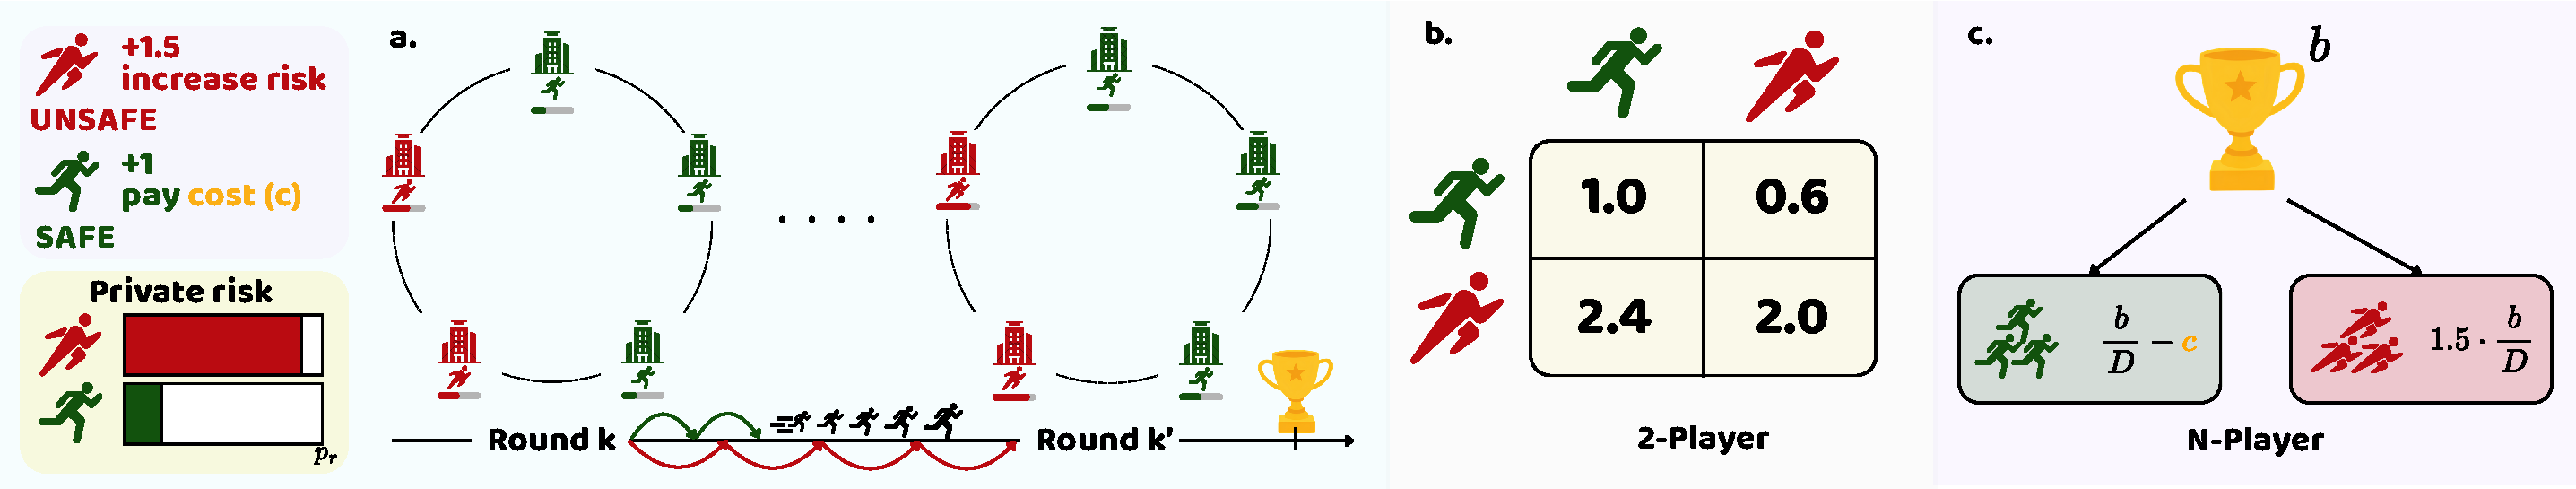
\includegraphics[width=\textwidth]{figures/AIRaceOverview.pdf}
  \caption{Overview of the AI-race mechanism shared by the two-player and $N$-player games. (a) Each round, every company advances along the track by choosing Safe (green, $+1$ progress, pays cost $c$) or Unsafe (red, $+1.5$ progress, increases private setback risk); the race ends after a hidden number of rounds, at which point terminal prize $B$ is awarded to the progress leader or divided among tied leaders. (b) The two-player stage-payoff matrix: own Safe/opponent Safe pays 1.0, own Safe/opponent Unsafe pays 0.6, own Unsafe/opponent Safe pays 2.4, and own Unsafe/opponent Unsafe pays 2.0. (c) The $N$-player stage-payoff rule: if $k$ of $N$ companies choose Safe, $D=k+s(N-k)$; each Safe-choosing company earns $b/D-c$ and each Unsafe-choosing company earns $s b/D$, where $b$ is the per-round benefit and is distinct from terminal prize $B$.}
  \label{fig:mechanism}
  \Description{Three-panel diagram of the AI-race mechanism. Panel a shows company icons moving around a circular track, with green Safe icons advancing one step and red Unsafe icons advancing one and a half steps while increasing a private risk bar; the track leads to terminal prize B after an unmarked number of rounds. Panel b shows the two-player payoff matrix as a two-by-two grid labelled Safe and Unsafe on each axis, with values 1.0, 0.6, 2.4, and 2.0. Panel c shows the $N$-player stage-payoff rule: if $k$ of $N$ companies choose Safe, $D=k+s(N-k)$; Safe receives $b/D-c$ and Unsafe receives $s b/D$. Lowercase $b$ denotes per-round benefit, not terminal prize $B$.}
\end{figure*}

% ARTWORK TODO: distinguish the true no-persona baseline from the neutral-placebo
% role sentence in panel (a), if the source artwork is regenerated.
\begin{figure*}[t]
  \centering
  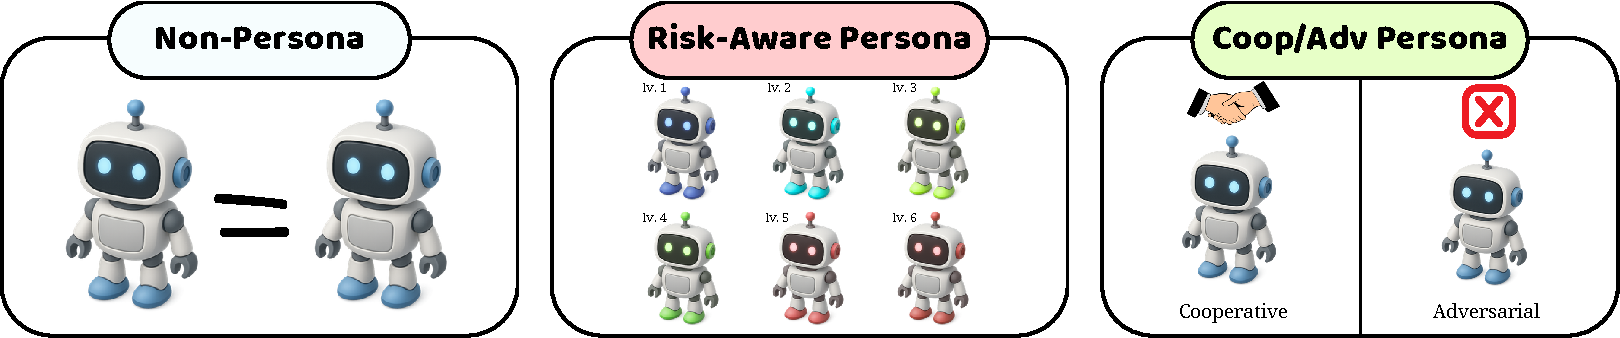
\includegraphics[width=0.7\textwidth]{figures/ExpOverview.pdf}
  \caption{Overview of the three persona-related framing families used to describe each company's executive. The canonical baseline contains no persona sentence; a separate neutral placebo uses a length-matched neutral sentence. The risk-aware family contains six levels adapted from the Eckel--Grossman gamble scale. The cooperative/adversarial family frames each seat as believing rival firms do better through mutual restraint or only at each other's expense. These are prompt conditions, not measured psychological traits.}
  \label{fig:persona}
  \Description{Three-panel illustration using simple robot mascots to represent company executives. Panel 1, non-persona, shows three identical robots labelled Company A, Company B, and Company C, indicating no persona text is applied. Panel 2, risk-aware persona, shows a colour gradient from lowest to highest risk acceptance above six robot figures labelled Level 1 through Level 6, each holding a different prop suggesting increasing risk tolerance, from crossed arms at level one to raised arms at level six. Panel 3, cooperative versus adversarial persona, shows two robots shaking hands under a green cooperative label with a handshake icon, and two robots with red eyes and crossed arms under a red adversarial label with a shield-and-cross icon.}
\end{figure*}

This study aims to determine whether large language model (LLM) agents can reproduce observable patterns of safety behaviour in an idealised AI race and whether these patterns remain stable as the competitive setting changes. We use a staged approach because an output does not by itself show that an agent has followed the rules or correctly represented the evolving state of the race. The analysis therefore begins with task-validity checks, proceeds to the two-player human benchmark, and then considers the exploratory $N$-player extension. This paper addresses the following research questions:
\begin{itemize}
    \item Can LLM agents reliably execute the rules and state transitions of the AI-race game?
    \item How are private risk, prior actions, race position, and early choices associated with \Unsafe{} play?
    \item How stable are these behavioural patterns across models, prompts, personas, and decoding protocols?
    \item How do group size and multiplayer race state relate to \Unsafe{} play in exploratory $N$-player settings?
\end{itemize}

\section{Preliminaries}
\label{sec:preliminaries}

We first specify the two-player game reproduced from \citet{falling_behind_unsafe} (\S\ref{sec:prelim-2p}), then its generalisation to $N>2$ companies (\S\ref{sec:prelim-np}). Every quantity that is not restated in \S\ref{sec:prelim-np}, namely the horizon, prize split, and private-risk formula, carries over unchanged from the two-player game; only the stage payoff changes shape (Figure~\ref{fig:mechanism}).

\subsection{Two-player game}
\label{sec:prelim-2p}

Two companies $i \in \{1,2\}$ play a repeated race. In every round $t$, both companies simultaneously choose an action $a_i^t \in \{S, U\}$ (Safe, Unsafe) and commit to it before either learns the other's choice for that round; only once both actions are committed does the round resolve (Figure~\ref{fig:mechanism}a). Resolution has two parts. First, Safe advances the company's cumulative progress by $\sigma(S)=1.0$ and Unsafe advances it by $\sigma(U)=1.5$, so Unsafe always closes the race faster; progress accumulates as $P_i^t = P_i^{t-1}+\sigma(a_i^t)$. Second, the round pays a stage payoff $\pi_i^t=\pi(a_i^t,a_{-i}^t)$, read off the fixed matrix (own action by row, opponent action by column, Figure~\ref{fig:mechanism}b):
\begin{equation}
    \pi = \begin{pmatrix} 1.0 & 0.6 \\ 2.4 & 2.0 \end{pmatrix}.
    \label{eq:2p-matrix}
\end{equation}
Unsafe strictly dominates Safe at the stage-game level (row 2 exceeds row 1 in both columns): the only cost of Unsafe development enters later, through accumulated private risk rather than through the round payoff itself.

The race lasts a minimum of $5$ rounds; after every completed round from round $5$ onward it terminates with probability $0.2$, giving an expected horizon $\mathbb{E}[T]=9$. Neither company is ever told the horizon in advance, so a company can never condition its action on knowing the current round is the last one (Figure~\ref{fig:mechanism}a). Termination then resolves in two further steps. First, the company with the higher cumulative progress $P_i^T$ is declared the winner of a prize $B=100$; if progress is exactly tied, the two companies split it $50/50$. Second, and only for that winner or tied winners, an accumulated private setback risk is drawn:
\begin{equation}
    q_i(T) = p_r^{\max} \cdot \frac{n_i^U(T)}{T}, q_i(T) \in [0,1], p_r^{\max}\in\{0.10,0.60,0.90\},
    \label{eq:risk}
\end{equation}
where $n_i^U(T)$ counts company $i$'s Unsafe choices over the whole race and $p_r^{\max}$ is a treatment-level constant, assigned once per race, that we vary across three risk levels. If the draw against $q_i(T)$ fails, that company's entire race payoff, every stage payoff it accumulated plus the prize, is zeroed; if it succeeds, the company keeps both. A company that ends behind is never subject to this draw at all: it keeps its accumulated stage payoffs regardless of how much Unsafe it played, but receives no share of the prize (Figure~\ref{fig:mechanism}a). This asymmetry, in which risk is built by both companies but realised only against whoever is ahead, is what makes Unsafe development a genuine gamble rather than a free speed advantage.

\subsection{$N$-player game}
\label{sec:prelim-np}

The $N$-player game keeps every element of \S\ref{sec:prelim-2p} unchanged (simultaneous sealed actions, progress increments $\sigma(S)=1.0$/$\sigma(U)=1.5$, the minimum-5-round hidden horizon, terminal prize $B=100$, and the risk formula, Equation~\ref{eq:risk}), but is played by $N\geq2$ companies indexed by $i\in\{1,\dots,N\}$ instead of exactly two, and the prize at round $T$ splits evenly among however many companies share the highest progress rather than only two. The engine supports $N\in\{2,3,4,5\}$; the current output covers $N=3$, while matched $N=4$ and $N=5$ conditions remain planned (Figure~\ref{fig:mechanism}c).

With more than two companies there is no single opponent to index a matrix against, so Equation~\ref{eq:2p-matrix} generalises to the $N$-player stage-payoff rule of \citet{to_regulate_or_not} (their Appendix~B), evaluated at $k^t \in \{0,1,\dots,N\}$, the number of companies (out of $N$) choosing Safe in round $t$. Therefore, every Safe-choosing company earns
% That original rule includes a further parameter $p_{fo}$, the probability that an Unsafe company is found out within the round and forfeits its benefit for it; we set $p_{fo}=0$ throughout, so a company's only cost for choosing Unsafe is the terminal private setback risk of Equation~\ref{eq:risk}, not an additional per-round detection risk. At $p_{fo}=0$, every Safe-choosing company earns
\begin{equation}
    \pi_{\text{Safe}}(k^t) = \frac{b}{k^t + s\,(N-k^t)} - c,
    \label{eq:np-safe}
\end{equation}
and every Unsafe-choosing company earns
\begin{equation}
    \pi_{\text{Unsafe}}(k^t) = s \cdot \frac{b}{k^t + s\,(N-k^t)},
    \label{eq:np-unsafe}
\end{equation}
with cost $c=1$, per-round benefit $b=4$, and speed $s=1.5$ fixed across all group sizes (the per-round benefit $b$ is distinct from terminal prize $B$, which is paid once, at the end of the race, not every round). Both payoffs depend on the \emph{group's} joint action counts, $k^t$ and $N-k^t$, not on any single rival's action, which is the structural difference from the two-player game: a company's stage payoff now moves with how many of its rivals, not which one, chose each action.

\subsection{Playground Simulation}

% To do Project contribution - need results%


% This document explains the main features of the `\texttt{aamas}'
% document class, which is essentially identical to the `\texttt{acmart}'
% document class provided by the ACM. The only difference is a minor
% modification to allow for the correct copyright attribution to IFAAMAS.
% For detailed documentation of the original document class, please refer
% to the relevant website maintained by the~ACM:
% %
% \begin{center}
% \url{https://www.acm.org/publications/proceedings-template}
% \end{center}
% %
% The first command in your source file should be either one of these:
% \begin{verbatim}
%     \documentclass[sigconf,anonymous]{aamas}
%     \documentclass[sigconf]{aamas}
% \end{verbatim}
% %
% The first variant should be
% used when you submit your paper for blind review; it will replace the names of the authors with the submission number.
% The second variant should be used for final papers.

% Make sure your paper includes the correct copyright information and
% the correct specification of the \emph{ACM Reference Format}. Both of
% these will be generated automatically if you include the correct
% \emph{copyright block} as shown in the source file of this document.

% Modifying the template---e.g., by changing margins, typeface sizes,
% line spacing, paragraph or list definitions---or making excessive use
% of the `\verb|\vspace|' command to manually adjust the vertical spacing
% between elements of your work is not allowed. You risk getting your
% submission rejected (or your final paper excluded from the proceedings)
% in case such modifications are discovered. The `\texttt{aamas}' document
% class requires the use of the \textit{Libertine} typeface family, which
% should be included with your \LaTeX\ installation. Please do not use
% other typefaces instead.

% Please consult the \emph{Call for Papers} for information on matters
% such as the page limit or anonymity requirements. It is available from
% the conference website:
% %
% \begin{center}
% \url{https://cyprusconferences.org/aamas2026/}
% \end{center}
% %
% To balance the columns on the final page of your paper, use the
% `\texttt{balance}' package and issue the `\verb|\balance|' command
%  somewhere in the text of what would be the first column of the last
%  page without balanced columns. This will be required for final papers.

%%%%%%%%%%%%%%%%%%%%%%%%%%%%%%%%%%%%%%%%%%%%%%%%%%%%%%%%%%%%%%%%%%%%%%%%

% \section{The Preamble}

% You will be assigned a submission number when you register the abstract
% of your paper on \textit{OpenReview}. Include this number in your
% document using the `\verb|\acmSubmissionID|' command.

% Then use the familiar commands to specify the title and authors of your
% paper in the preamble of the document. The title should be appropriately
% capitalised (meaning that every `important' word in the title should
% start with a capital letter). For the final version of your paper, make
% sure to specify the affiliation and email address of each author using
% the appropriate commands. Specify an affiliation and email address
% separately for each author, even if two authors share the same
% affiliation. You can specify more than one affiliation for an author by
% using a separate `\verb|\affiliation|' command for each affiliation.

% Provide a short abstract using the `\texttt{abstract}' environment.

% Finally, specify a small number of keywords characterising your work,
% using the `\verb|\keywords|' command.

% %%%%%%%%%%%%%%%%%%%%%%%%%%%%%%%%%%%%%%%%%%%%%%%%%%%%%%%%%%%%%%%%%%%%%%%%

% \section{The Body of the Paper}

% For help with typesetting the body of your paper in \LaTeX\@, please
% make use of the familiar resources~\cite{Lam94}. In this section we
% merely highlight a few specific features.

% \subsection{Mathematical Expressions}

% You can typeset all sorts of in-line mathematical expressions
% with the usual \verb|$...$| construct, as in
% $\Diamond\Diamond\varphi \rightarrow \Diamond\varphi$ or
% $\boldsymbol{R} = (R_1,\ldots,R_n)$.
% For more complex expressions, it may often be preferable to use one of
% the various equation-type environments available in \LaTeX\@, as shown
% in the following example:
% %
% \begin{eqnarray}
% Z_i & = & \frac{u_i(x_i) - u_i(x_{-i})}{u_i(x_i)}
% \end{eqnarray}
% %
% Here is a second example for an equation:
% %
% \begin{eqnarray}\label{eq:vcg}
% p_i(\boldsymbol{\hat{v}}) & = &
% \sum_{j \neq i} \hat{v}_j(f(\boldsymbol{\hat{v}}_{-i})) -
% \sum_{j \neq i} \hat{v}_j(f(\boldsymbol{\hat{v}}))
% \end{eqnarray}
% %
% Use the usual combination of `\verb|\label|' and `\verb|\ref|' to refer
% to numbered equations, such as Equation~(\ref{eq:vcg}) above. Of course,
% introducing numbers in the first place is only helpful if you in fact
% need to refer back to the equation in question elsewhere in the paper.


% \subsection{Tables and Figures}

% Use the `\texttt{table}' environment (or its variant `\texttt{table*}')
% in combination with the `\texttt{tabular}' environment to typeset tables
% as floating objects. The `\texttt{aamas}' document class includes the
% `\texttt{booktabs}' package for preparing high-quality tables. Tables
% are often placed at the top of a page near their initial cite, as done
% here for Table~\ref{tab:locations}.

% \begin{table}[t]
% 	\caption{Locations of the first five editions of AAMAS}
% 	\label{tab:locations}
% 	\begin{tabular}{rll}\toprule
% 		\textit{Year} & \textit{City} & \textit{Country} \\ \midrule
% 		2002 & Bologna & Italy \\
% 		2003 & Melbourne & Australia \\
% 		2004 & New York City & USA \\
% 		2005 & Utrecht & The Netherlands \\
% 		2006 & Hakodate & Japan \\ \bottomrule
% 	\end{tabular}
% \end{table}

% The caption of a table should be placed \emph{above} the table.
% Always use the `\verb|\midrule|' command to separate header rows from
% data rows, and use it only for this purpose. This enables assistive
% technologies to recognise table headers and support their users in
% navigating tables more easily.

% %%% The following command should be issued somewhere in the first column
% %%% of the final page of your paper.
% \balance

% Use the `\texttt{figure}' environment for figures. If your figure
% contains third-party material, make sure to clearly identify it as such.
% Every figure should include a caption, and this caption should be placed
% \emph{below} the figure itself, as shown here for Figure~\ref{fig:logo}.

% \begin{figure}[h]
%   \centering
%   
\includegraphics[width=0.75\linewidth]{aamas2026logo}
%   \caption{The logo of AAMAS 2026}
%   \label{fig:logo}
%   \Description{Logo of AAMAS 2026 -- The 25th International Conference on Autonomous Agents and Multiagent Systems.}
% \end{figure}

% In addition, every figure should also have a figure description, unless
% it is purely decorative. Use the `\verb|\Description|' command for this
% purpose. These descriptions will not be printed but can be used to
% convey what's in an image to someone who cannot see it. They are also
% used by search engine crawlers for indexing images, and when images
% cannot be loaded. A figure description must consist of unformatted plain
% text of up to 2000~characters. For example, the definition of
% Figure~\ref{fig:logo} in the source file of this document includes the
% following description: ``Logo of AAMAS 2026 -- The 25th International Conference on Autonomous Agents and Multiagent Systems.'' For more information on how best to write figure descriptions
% and why doing so is important, consult the information available here:
% %
% \begin{center}
% \url{https://www.acm.org/publications/taps/describing-figures/}
% \end{center}
% %
% The use of colour in figures and graphs is permitted, provided they
% remain readable when printed in greyscale and provided they are
% intelligible also for people with a colour vision deficiency.

% %%%%%%%%%%%%%%%%%%%%%%%%%%%%%%%%%%%%%%%%%%%%%%%%%%%%%%%%%%%%%%%%%%%%%%%%

% \section{Citations and References}

% The use of the \BibTeX\ to prepare your list of references is highly
% recommended. To include the references at the end of your document, put
% the following two commands just before the `\verb|\end{document}|'
% command in your source file:
% %
% \begin{verbatim}
% TODO for camera-ready: place \balance in the first column of the final page
% after the complete manuscript has been compiled and its page breaks are known.
%    \bibliographystyle{ACM-Reference-Format}
%    \bibliography{sample}
% \end{verbatim}
% %
% Here we assume that `\texttt{sample.bib}' is the name of your
% \BibTeX\ file. Use the `\verb|\cite|' command to produce citations
% to your references. Here are a few examples for citations of journal
% articles~\cite{GrKr96,WoJe95}, books~\cite{Knu97}, articles in
% conference proceedings~\cite{Hag1993}, technical reports~\cite{Har78},
% Master's and PhD theses~\cite{Ani03,Cla85}, online videos~\cite{Oba08},
% datasets~\cite{AnMC13}, and patents~\cite{Sci09}. Both citations and
% references are numbered by default.

% Make sure you provide complete and correct bibliographic information
% for all your references, and list authors with their full names
% (``Donald E.\ Knuth'') rather than just initials (``D.\ E.\ Knuth'').

% %%%%%%%%%%%%%%%%%%%%%%%%%%%%%%%%%%%%%%%%%%%%%%%%%%%%%%%%%%%%%%%%%%%%%%%%

% %%% The acknowledgments section is defined using the "acks" environment
% %%% (rather than an unnumbered section). The use of this environment
% %%% ensures the proper identification of the section in the article
% %%% metadata as well as the consistent spelling of the heading.

% \begin{acks}
% If you wish to include any acknowledgments in your paper (e.g., to
% people or funding agencies), please do so using the `\texttt{acks}'
% environment. Note that the text of your acknowledgments will be omitted
% if you compile your document with the `\texttt{anonymous}' option.
% \end{acks}

%%%%%%%%%%%%%%%%%%%%%%%%%%%%%%%%%%%%%%%%%%%%%%%%%%%%%%%%%%%%%%%%%%%%%%%%

%%% The next two lines define, first, the bibliography style to be
%%% applied, and, second, the bibliography file to be used.

\bibliographystyle{ACM-Reference-Format}
% \bibliography{sample}
\bibliography{references}

%%%%%%%%%%%%%%%%%%%%%%%%%%%%%%%%%%%%%%%%%%%%%%%%%%%%%%%%%%%%%%%%%%%%%%%%

\end{document}

%%%%%%%%%%%%%%%%%%%%%%%%%%%%%%%%%%%%%%%%%%%%%%%%%%%%%%%%%%%%%%%%%%%%%%%%
